\documentclass[border=10pt]{standalone}

\usepackage{tikz}
\usepackage{tikzsymbols}
\usetikzlibrary{calc,patterns,shapes.geometric}

\def\centerarc[#1](#2)(#3:#4:#5){\draw[#1] ($(#2)+({#5*cos(#3)},{#5*sin(#3)})$) arc (#3:#4:#5);}

\begin{document}
	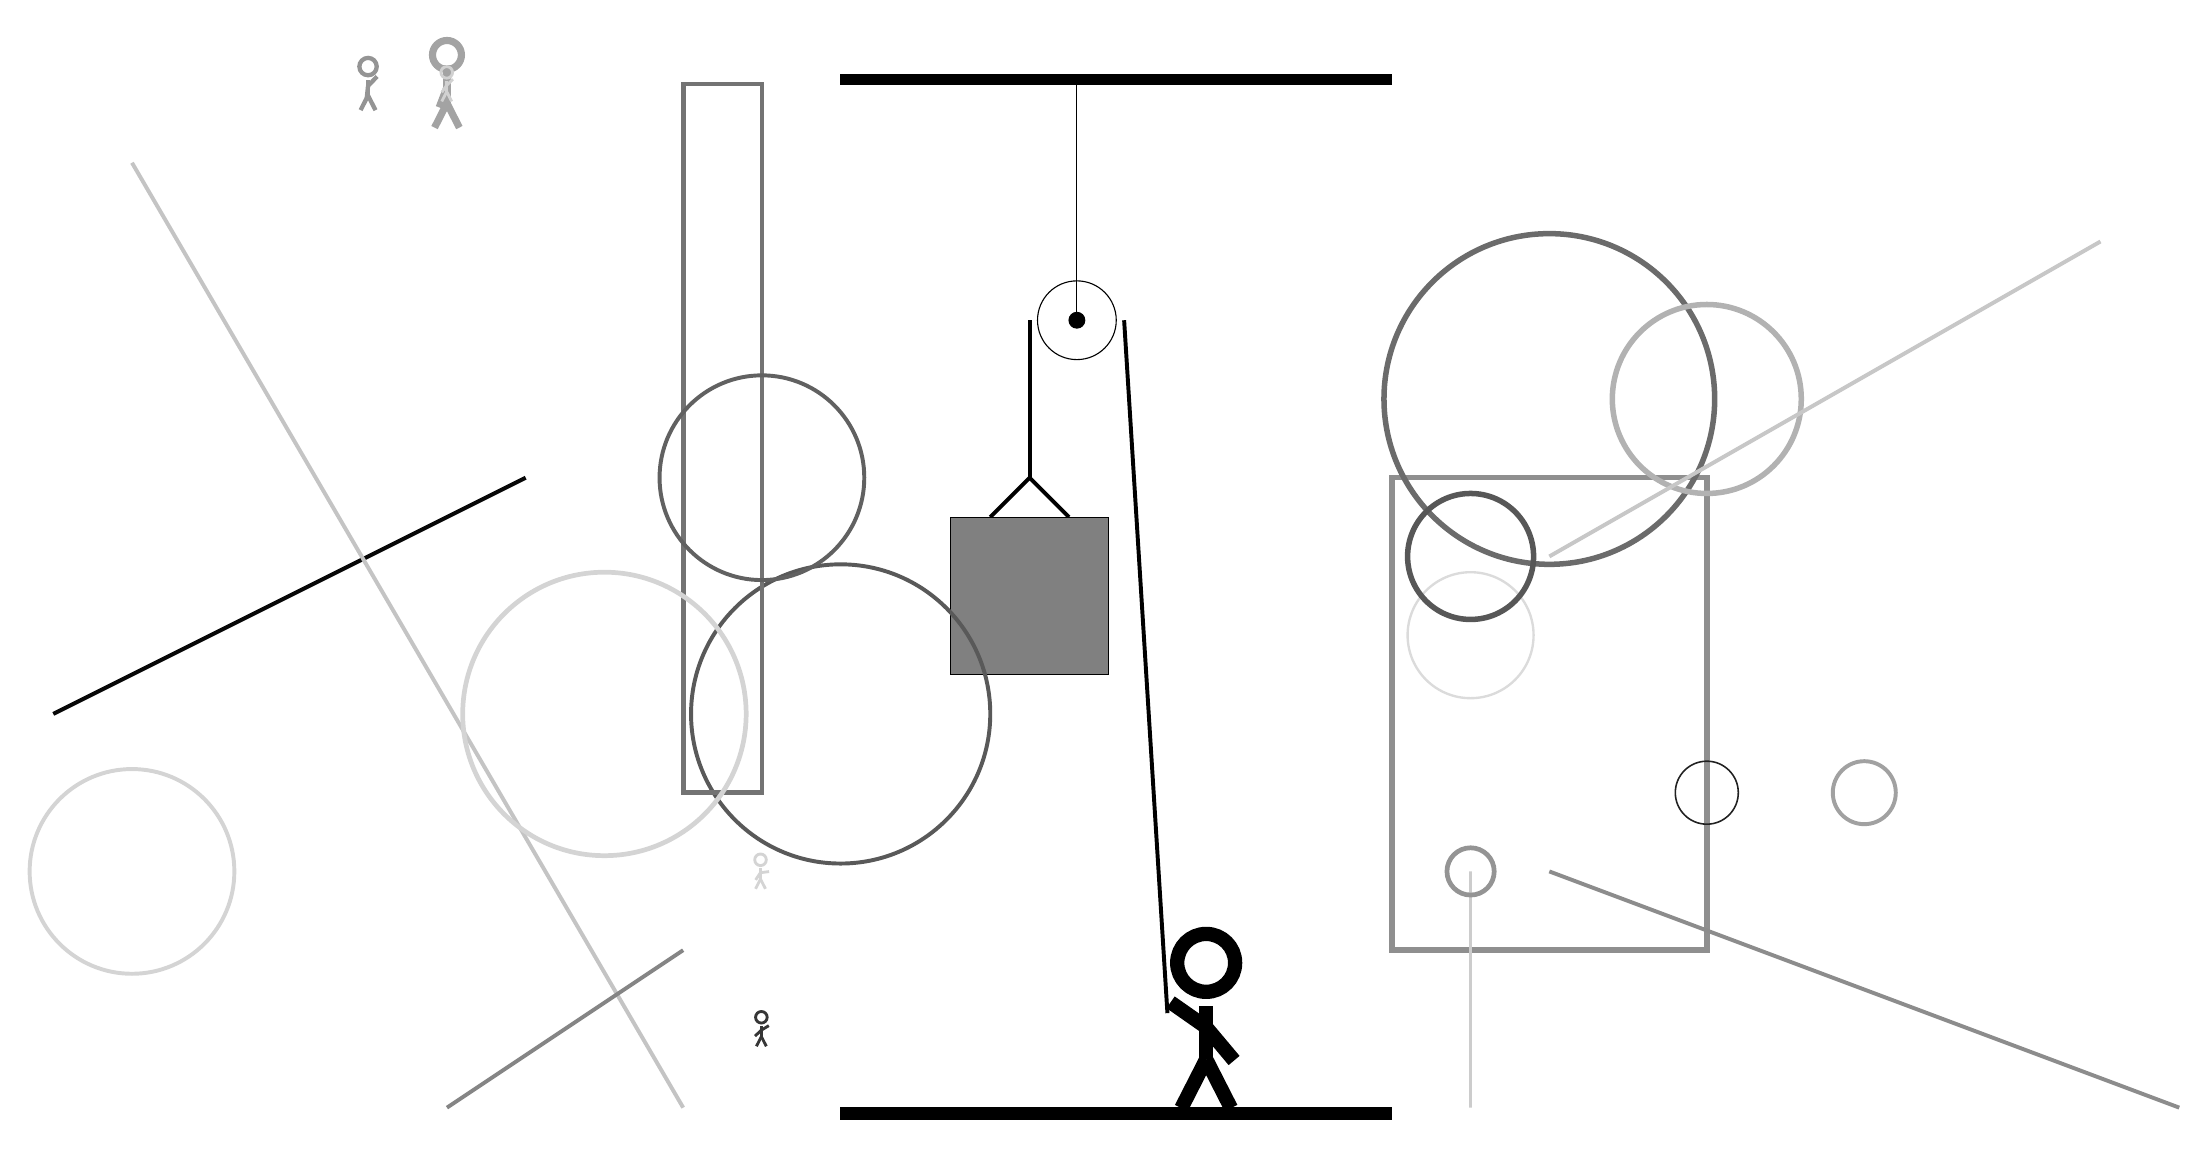
\begin{tikzpicture}
		%%%%% START %%%%%
		
		\draw[fill=black] (-2, 10) rectangle (5, 10.125);
		
		\draw (1, 7) circle (0.5);
		\draw[fill=black] (1, 7) circle (0.1);
		\draw (1, 10) -- (1, 7);
		
		\draw[line width=0.5mm] (-0.1, 4.5) -- (0.4, 5.0) -- (0.9, 4.5);
		\draw[fill=black!50] (-0.6, 4.5) rectangle (1.4, 2.5);
		
		\draw[line width=0.5mm] (0.4, 7) -- (0.4, 5.0);
		\centerarc[line width=0.5mm](1, 7)(0:180:0.6);
		\draw[line width=0.5mm](1.6, 7) -- (2.15, -1.8);
		
		\draw[line width=0.7mm, color=black!44] (5, -1) rectangle (9, 5);
		
		\draw[line width=0.5mm, color=black!97](-6, 5) -- (-12, 2);
		\node[line width=0.4mm, color=black!36] at (-7, 10) {\Strichmaxerl[5][69][90]};
		\draw [line width=0.3mm, color=black!14](6, 3) circle (0.8);
		
		\draw [line width=0.7mm, color=black!58](7, 6) circle (2.1);
		
		\draw[line width=0.4mm, color=black!20] (6, 0) rectangle (6, -3);
		\draw[line width=0.5mm, color=black!45](7, 0) -- (15, -3);
		
		\draw [line width=0.7mm, color=black!30](9, 6) circle (1.2);
		\draw [line width=0.7mm, color=black!66](6, 4) circle (0.8);
		\draw[line width=0.5mm, color=black!23](-4, -3) -- (-11, 9);
		\node[line width=0.3mm, color=black!79] at (-3, -2) {\Strichmaxerl[2][43][31]};
		\draw [line width=0.5mm, color=black!17](-11, 0) circle (1.3);
		\draw [line width=0.5mm, color=black!65](-2, 2) circle (1.9);
		\draw[line width=0.6mm, color=black!55] (-4, 1) rectangle (-3, 10);
		\draw [line width=0.5mm, color=black!62](-3, 5) circle (1.3);
		\draw [line width=0.6mm, color=black!42](6, 0) circle (0.3);
		\node[line width=0.6mm, color=black!17] at (-3, 0) {\Strichmaxerl[2][56][7]};
		\draw [line width=0.2mm, color=black!87](9, 1) circle (0.4);
		\draw [line width=0.5mm, color=black!37](11, 1) circle (0.4);
		
		\node[line width=0.7mm, color=black!18] at (-7, 10) {\Strichmaxerl[2][55][44]};
		\draw[line width=0.5mm, color=black!22](7, 4) -- (14, 8);
		
		\draw [line width=0.6mm, color=black!17](-5, 2) circle (1.8);
		
		\node[line width=0.3mm, color=black!42] at (-8, 10) {\Strichmaxerl[3][84][46]};
		\draw[line width=0.5mm, color=black!48](-7, -3) -- (-4, -1);
		
		\node at (2.6, -1.9) {\Strichmaxerl[10][-35][-50]};
		
		\draw[fill=black] (-2, -3) rectangle (5, -3.15);
		
		%%%%% END %%%%%
	\end{tikzpicture}
\end{document}